\section{Jev with Qwen in the loop}
\label{sec:escalation}

A class distribution also says when a second opinion is worth paying for. We keep Jev's
prediction when its maximum class probability is at least a threshold $t$ and take Qwen's
otherwise. The reported point uses the $t$ that maximizes macro-F1 on validation items only,
with ties broken towards fewer escalations; everything is computed from saved predictions
(Figure~\ref{fig:escalation}; Appendix~\ref{app:escalation} lists the validation items).

\begin{figure}[t]
  \centering
  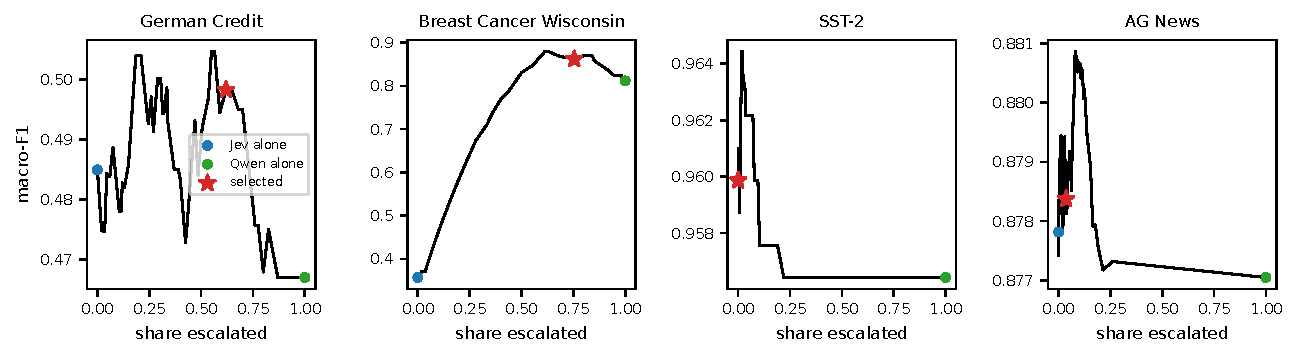
\includegraphics[width=\linewidth]{generated/figs/escalation}
  \caption{Macro-F1 of the ensemble against the share of evaluation items escalated to Qwen
    (first split repeat for the tabular datasets). The star marks the validation-selected
    threshold.}
  \label{fig:escalation}
\end{figure}

\begin{table}[t]
  \caption{Escalation of low-confidence Jev predictions to Qwen3.6-27B: macro-F1 of each model
    alone and of the ensemble at the validation-selected threshold $t$, the share of items
    escalated, the cost per 1,000 predictions, and the Jev errors at its highest reported
    confidence, which no threshold can reach without escalating every item at that confidence.}
  \label{tab:escalation}
  \centering\small
  \setlength{\tabcolsep}{4pt}
  \fittable{\begin{tabular}{lccccccr}
\toprule
Dataset & Jev & Qwen & $t$ & Share & Ensemble & USD/1,000 & Unreachable \\
\midrule
German Credit & 0.467\,{\scriptsize$\pm$0.019} & 0.457\,{\scriptsize$\pm$0.025} & 0.88 & 0.58 & 0.478\,{\scriptsize$\pm$0.029} & 0.421 & 5 of 103 \\
Breast Cancer Wisconsin & 0.343\,{\scriptsize$\pm$0.019} & 0.783\,{\scriptsize$\pm$0.029} & 0.85 & 0.69 & 0.856\,{\scriptsize$\pm$0.027} & 0.950 & 0 of 66 \\
SST-2 & 0.960 & 0.956 & 0.00 & 0.00 & 0.960 & 0.015 & 5 of 35 \\
AG News & 0.878 & 0.877 & 0.65 & 0.04 & 0.878 & 0.040 & 307 of 923 \\
\bottomrule
\end{tabular}
}
\end{table}

The outcome depends on what Jev's confidence knows (Table~\ref{tab:escalation}). On Breast Cancer
Wisconsin the ensemble beats both of its members: macro-F1 \EscFOneWdbc{} against
\EscJevFOneWdbc{} for Jev and \EscQwenFOneWdbc{} for Qwen, escalating \EscShareWdbc{} of the
items. Jev's confident predictions there are mostly right, and the ones it is unsure of are
better left to Qwen. On German Credit, where neither model ranks the rows, escalating
\EscShareGerman{} of them moves macro-F1 only from \EscJevFOneGerman{} to \EscFOneGerman. On
SST-2 the selected threshold escalates nothing. On AG News \EscShareAgnews{} of the items are
escalated and macro-F1 stays at \EscFOneAgnews: the two models are equally accurate, and
\EscUnreachableAgnews{} of Jev's \EscErrorsAgnews{} errors carry its highest reported confidence,
shared by \EscShareAtMaxAgnews{} of all items. Escalation is paid for at Qwen's price: USD
\EscCostPerKWdbc{} per 1,000 predictions on Breast Cancer Wisconsin against USD
\CostPerKJevWdbc{} for Jev alone.
